% !TEX root = ../PolycopiePremiere2627.tex

\chapter{Variations quadratiques}

\noindent\textbf{Activité}

Depuis un plongeoir, une plongeuse s'élance dans une piscine. On modélise sa hauteur au-dessus de l'eau, en mètres, par la fonction $h$ définie pour $t\in[0\ ;\ 4,1]$ ($t$ étant le temps écoulé, en secondes, depuis le début du saut) par :
\[h(t)=-5t^2+20t+1\]

\begin{enumerate}
    \item Compléter le tableau de valeurs suivant.

    \begin{center}
        \begin{tabular}{|c|c|c|c|c|c|}
            \hline
            $t$ & 0 & 1 & 2 & 3 & 4 \\
            \hline
            $h(t)$ & \textcolor{J1}{1} & \textcolor{J1}{16} & \textcolor{J1}{21} & \textcolor{J1}{16} & \textcolor{J1}{1} \\
            \hline
        \end{tabular}
    \end{center}

    \item Placer les points correspondants sur le graphique suivant.

    \begin{center}
        \begin{tikzpicture}[scale=1,very thick]
            \begin{axis}[
                    xscale=1.6,
                    yscale=.35,
                    xmin=0,
                    xmax=4.5,
                    ymin=0,
                    ymax=23,
                    ultra thick,
                    axis lines=middle,
                    enlargelimits=upper,
                    xtick={0,1,...,4},
                    ytick={0,5,...,20},
                    major grid style={black, thick},
                    grid=both,
                    clip=false,
                ]
                \draw (axis cs:0, 0) node[below left]{$0$};
                \draw (axis cs:4.5, 0) node[below=2pt]{$t$ (s)};
                \draw (axis cs:0, 23) node[right=2pt]{$h(t)$ (m)};
                \addplot[only marks, mark=x, J1, thick] coordinates {(0,1) (1,16) (2,21) (3,16) (4,1)};
            \end{axis}
        \end{tikzpicture}%
    \end{center}

    \item Quelle semble être la hauteur maximale atteinte par la plongeuse ? À quel instant ?

    \textcolor{J1}{La hauteur maximale semble être de 21 m, atteinte à l'instant $t=2$ s.}
    \item Que remarquez-vous concernant la disposition des points ?

    \textcolor{J1}{Le nuage de points n'est pas aligné (ce n'est donc pas un modèle linéaire) : il semble symétrique par rapport à la droite verticale d'équation $t=2$.}
\end{enumerate}

\pagebreak

\section{Fonction polynôme du second degré}

\Dfn{On appelle \textcolor{J1}{fonction polynôme du second degré} (ou \textcolor{J1}{trinôme du second degré}) toute fonction $f$ définie sur $\R$ pouvant s'écrire sous la forme
\[f(x)=ax^2+bx+c\]
où $a$, $b$ et $c$ sont des nombres réels, avec $a\neq0$. Sa courbe représentative s'appelle une \textcolor{J1}{parabole}.}

\Exemple{Parmi les fonctions suivantes, lesquelles sont des fonctions polynômes du second degré ? Le cas échéant, donner les valeurs de $a$, $b$ et $c$.
\begin{enumerate}
    \item $f(x)=3x^2-5x+2$ : \textcolor{J1}{oui, avec $a=3$, $b=-5$, $c=2$.}
    \item $g(x)=2x-7$ : \textcolor{J1}{non, $g$ est une fonction affine (pas de terme en $x^2$).}
    \item $h(x)=-x^2+4$ : \textcolor{J1}{oui, avec $a=-1$, $b=0$, $c=4$.}
    \item $k(x)=x^3-x^2+1$ : \textcolor{J1}{non, $k$ contient un terme en $x^3$.}
\end{enumerate}}

\Prp[Cas particulier $f(x)=ax^2$]{La courbe représentative de $f:x\mapsto ax^2$ est une parabole de sommet $O(0\ ;\ 0)$, symétrique par rapport à l'axe des ordonnées. Selon le signe de $a$ :
\begin{itemize}
    \item si $a>0$, la parabole est tournée vers le haut, et $f$ admet un \textcolor{J1}{minimum} en $0$, égal à $0$ ;
    \item si $a<0$, la parabole est tournée vers le bas, et $f$ admet un \textcolor{J1}{maximum} en $0$, égal à $0$.
\end{itemize}}

\begin{center}
    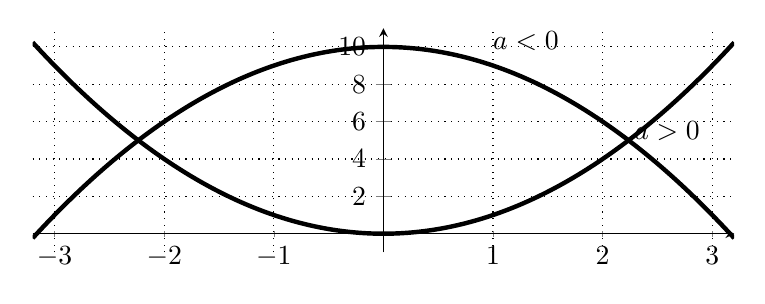
\begin{tikzpicture}
        \begin{axis}[
                xscale=1.3,
                yscale=.5,
                domain=-3.2:3.2,
                axis lines=middle,
                xtick={-3,-2,...,3},
                ytick={0,2,...,10},
                ymin=-1,
                ymax=11,
                clip=true,
                grid style={dotted,black},
                grid=both,
            ]
            \addplot[black, ultra thick, samples=100, smooth]{x^2};
            \addplot[black, ultra thick, samples=100, smooth]{-x^2+10};
            \draw (axis cs:2.2,5.5) node[right]{$a>0$};
            \draw (axis cs:1.3,9.3) node[above]{$a<0$};
        \end{axis}
    \end{tikzpicture}
\end{center}

\Prp[Tableau de variations de $x\mapsto ax^2$]{
\begin{center}
    \begin{minipage}{0.46\linewidth}
        \centering\textbf{Si $a>0$}

        \begin{tikzpicture}
            \tkzTabInit[lgt=2,espcl=2.5]{$x$/1,$f(x)$/2}{$-\infty$,$0$,$+\infty$}
            \tkzTabVar{-/$+\infty$,+/$0$,+/$+\infty$}
        \end{tikzpicture}
    \end{minipage}\hfill
    \begin{minipage}{0.46\linewidth}
        \centering\textbf{Si $a<0$}

        \begin{tikzpicture}
            \tkzTabInit[lgt=2,espcl=2.5]{$x$/1,$f(x)$/2}{$-\infty$,$0$,$+\infty$}
            \tkzTabVar{+/$-\infty$,-/$0$,-/$-\infty$}
        \end{tikzpicture}
    \end{minipage}
\end{center}}

\Prp[Fonctions de la forme $x\mapsto ax^2+c$]{La courbe de $f:x\mapsto ax^2+c$ s'obtient en translatant verticalement celle de $x\mapsto ax^2$ de $c$ unités. Son sommet est le point $S(0\ ;\ c)$, et son axe de symétrie reste l'axe des ordonnées (la droite d'équation $x=0$).}

\Exemple{On considère les fonctions $f:x\mapsto2x^2-3$ et $g:x\mapsto-0,5x^2+4$.
\begin{enumerate}
    \item Donner le sommet et l'axe de symétrie de chacune des deux courbes.

    \textcolor{J1}{Pour $f$ : sommet $S_f(0\ ;\ -3)$, axe de symétrie d'équation $x=0$. Pour $g$ : sommet $S_g(0\ ;\ 4)$, axe de symétrie d'équation $x=0$.}
    \item $f$ et $g$ admettent-elles chacune un minimum ou un maximum ?

    \textcolor{J1}{$f$ admet un minimum, car $a=2>0$ : il est égal à $-3$. $g$ admet un maximum, car $a=-0,5<0$ : il est égal à $4$.}
\end{enumerate}}

\section{Sommet et axe de symétrie de \texorpdfstring{$f(x)=ax^2+bx+c$}{f(x)=ax²+bx+c}}

\Prp{La courbe représentative d'une fonction polynôme du second degré $f:x\mapsto ax^2+bx+c$ est une parabole tournée vers le haut si $a>0$, vers le bas si $a<0$. Elle possède un axe de symétrie vertical, qui passe par le point le plus bas (ou le plus haut) de la courbe, appelé \textcolor{J1}{sommet} de la parabole.}

\ANoter{Contrairement au cas particulier $x\mapsto ax^2+c$, l'axe de symétrie de $f(x)=ax^2+bx+c$ n'est en général plus l'axe des ordonnées : il faut le déterminer.}

\Exemple{\label{ex:sommet}On considère la fonction $f$ définie sur $\R$ par $f(x)=x^2-6x+5$.

\medskip

\textbf{Etape 1} : on remarque que $f(0)=5$, et on cherche un autre nombre $x_0$ tel que $f(x_0)=5$ : son symétrique par rapport à l'axe.\\
\textcolor{J1}{$f(x)=5 \Longleftrightarrow x^2-6x+5=5 \Longleftrightarrow x^2-6x=0 \Longleftrightarrow x(x-6)=0$, donc $x=0$ ou $x=6$. Les points d'abscisses $0$ et $6$ ont donc la même image, $5$.}

\medskip

\textbf{Etape 2} : l'axe de symétrie de la parabole passe par le milieu de ces deux abscisses.\\
\textcolor{J1}{L'axe de symétrie a pour équation $x=\dfrac{0+6}{2}=3$.}

\medskip

\textbf{Etape 3} : le sommet de la parabole est le point de la courbe dont l'abscisse est celle de l'axe de symétrie.\\
\textcolor{J1}{$f(3)=9-18+5=-4$, donc le sommet est le point $S(3\ ;\ -4)$.}

\medskip

\textbf{Etape 4} : comme $a=1>0$, la parabole est tournée vers le haut : $f$ est décroissante jusqu'au sommet, puis croissante.\\
\textcolor{J1}{
\begin{center}
    \begin{tikzpicture}
        \tkzTabInit[lgt=2,espcl=2.5]{$x$/1,$f(x)$/2}{$-\infty$,$3$,$+\infty$}
        \tkzTabVar{-/$+\infty$,+/$-4$,+/$+\infty$}
    \end{tikzpicture}
\end{center}
}

\begin{center}
    \begin{tikzpicture}
        \begin{axis}[
                xscale=1.1,
                yscale=.5,
                domain=-0.5:6.5,
                axis lines=middle,
                xtick={0,1,...,6},
                ytick={-4,-2,...,8},
                ymin=-5,
                ymax=9,
                clip=false,
                grid style={dotted,black},
                grid=both,
            ]
            \addplot[black, ultra thick, samples=100, smooth]{x^2-6*x+5};
            \addplot[only marks, mark=*, J1] coordinates {(3,-4)};
            \draw[J1, dashed] (axis cs:3,-5) -- (axis cs:3,9);
            \draw (axis cs:3,-4) node[right=6pt]{$S(3\,;\,-4)$};
        \end{axis}
    \end{tikzpicture}
\end{center}}

\Exemple{Reprendre la méthode de l'exemple \ref{ex:sommet} pour déterminer le sommet et les variations de $g(x)=-2x^2+8x+1$.

\textcolor{J1}{$g(0)=1$. On résout $g(x)=1 \Longleftrightarrow -2x^2+8x+1=1 \Longleftrightarrow -2x^2+8x=0 \Longleftrightarrow -2x(x-4)=0$, donc $x=0$ ou $x=4$. L'axe de symétrie a pour équation $x=\dfrac{0+4}{2}=2$. Or $g(2)=-8+16+1=9$, donc le sommet est $S(2\ ;\ 9)$. Comme $a=-2<0$, $g$ est croissante jusqu'au sommet, puis décroissante, avec un maximum égal à $9$.}}

\section{Forme factorisée : racines et signe}

\Dfn{Lorsqu'un polynôme du second degré $f(x)=ax^2+bx+c$ s'écrit sous la forme
\[f(x)=a(x-x_1)(x-x_2)\]
on dit qu'il est écrit sous \textcolor{J1}{forme factorisée}. Les nombres $x_1$ et $x_2$ sont alors les \textcolor{J1}{racines} du polynôme, c'est-à-dire les solutions de l'équation $f(x)=0$.}

\ANoter{Retrouver la forme factorisée d'un polynôme du second degré à partir de sa forme développée n'est, en général, pas au programme de cette année (elle fait appel au discriminant) : elle sera le plus souvent donnée dans l'énoncé, ou obtenue par une factorisation simple (facteur commun, identité remarquable).}

\Prp[Résolution par produit nul]{Un produit de facteurs est nul si et seulement si l'un au moins de ses facteurs est nul. Ainsi, les solutions de l'équation $a(x-x_1)(x-x_2)=0$ (avec $a\neq0$) sont exactement $x_1$ et $x_2$.}

\Exemple{Donner les racines du polynôme $f(x)=3(x+2)(x-5)$.

\textcolor{J1}{$f(x)=0 \Longleftrightarrow x+2=0$ ou $x-5=0 \Longleftrightarrow x=-2$ ou $x=5$. Les racines de $f$ sont donc $-2$ et $5$.}}

\Exemple{Factoriser $g(x)=2x^2-8x$ à l'aide d'un facteur commun, puis donner ses racines.

\textcolor{J1}{$g(x)=2x(x-4)$, sous forme factorisée avec $x_1=0$ et $x_2=4$ : ce sont les racines de $g$.}}

\Prp[Signe d'un polynôme du second degré factorisé]{Soit $f(x)=a(x-x_1)(x-x_2)$ un polynôme du second degré factorisé, avec $x_1\leq x_2$. Alors $f(x)$ est :
\begin{itemize}
    \item du signe de $a$ à l'extérieur des racines, c'est-à-dire sur $\left]-\infty\ ;\ x_1\right[$ et sur $\left]x_2\ ;\ +\infty\right[$ ;
    \item du signe opposé à $a$ entre les racines, c'est-à-dire sur $\left]x_1\ ;\ x_2\right[$ ;
    \item nul en $x_1$ et en $x_2$.
\end{itemize}}

\Exemple{Dressons le tableau de signes de $f(x)=-2(x+1)(x-4)$ sur $\R$.

\medskip

\textbf{Etape 1} : on détermine les racines, c'est-à-dire les valeurs qui annulent chaque facteur.\\
\textcolor{J1}{$x+1=0 \Longleftrightarrow x=-1$ \qquad et \qquad $x-4=0 \Longleftrightarrow x=4$.}

\medskip

\textbf{Etape 2} : on applique la propriété précédente, avec $a=-2<0$.

\begin{center}
    \begin{tikzpicture}
        \tkzTabInit[lgt=3,espcl=2.5]
          {$x$ / 1 , Signe de $f(x)$ / 1}
          {$-\infty$, \textcolor{J1}{$-1$}, \textcolor{J1}{$4$}, $+\infty$}
        \tkzTabLine{, \color{J1}-, \color{J1}0, \color{J1}+, \color{J1}0, \color{J1}-, }
    \end{tikzpicture}
\end{center}

\textcolor{J1}{$f$ est donc négative sur $\left]-\infty\ ;\ -1\right]$ et sur $\left[4\ ;\ +\infty\right[$, et positive sur $\left[-1\ ;\ 4\right]$ --- ce qui est cohérent avec $a=-2<0$ (signe de $a$ à l'extérieur des racines, signe opposé entre les racines).}}

\ANoter{Le signe d'un polynôme du second degré renseigne sur la position de sa parabole par rapport à l'axe des abscisses : la courbe est au-dessus de l'axe là où $f$ est positive, en dessous là où $f$ est négative, et coupe l'axe en ses racines.}
